\section{The Limits and Opportunities of Acceleration} \label{sec:limits}

\begin{figure}
  \begin{center}
    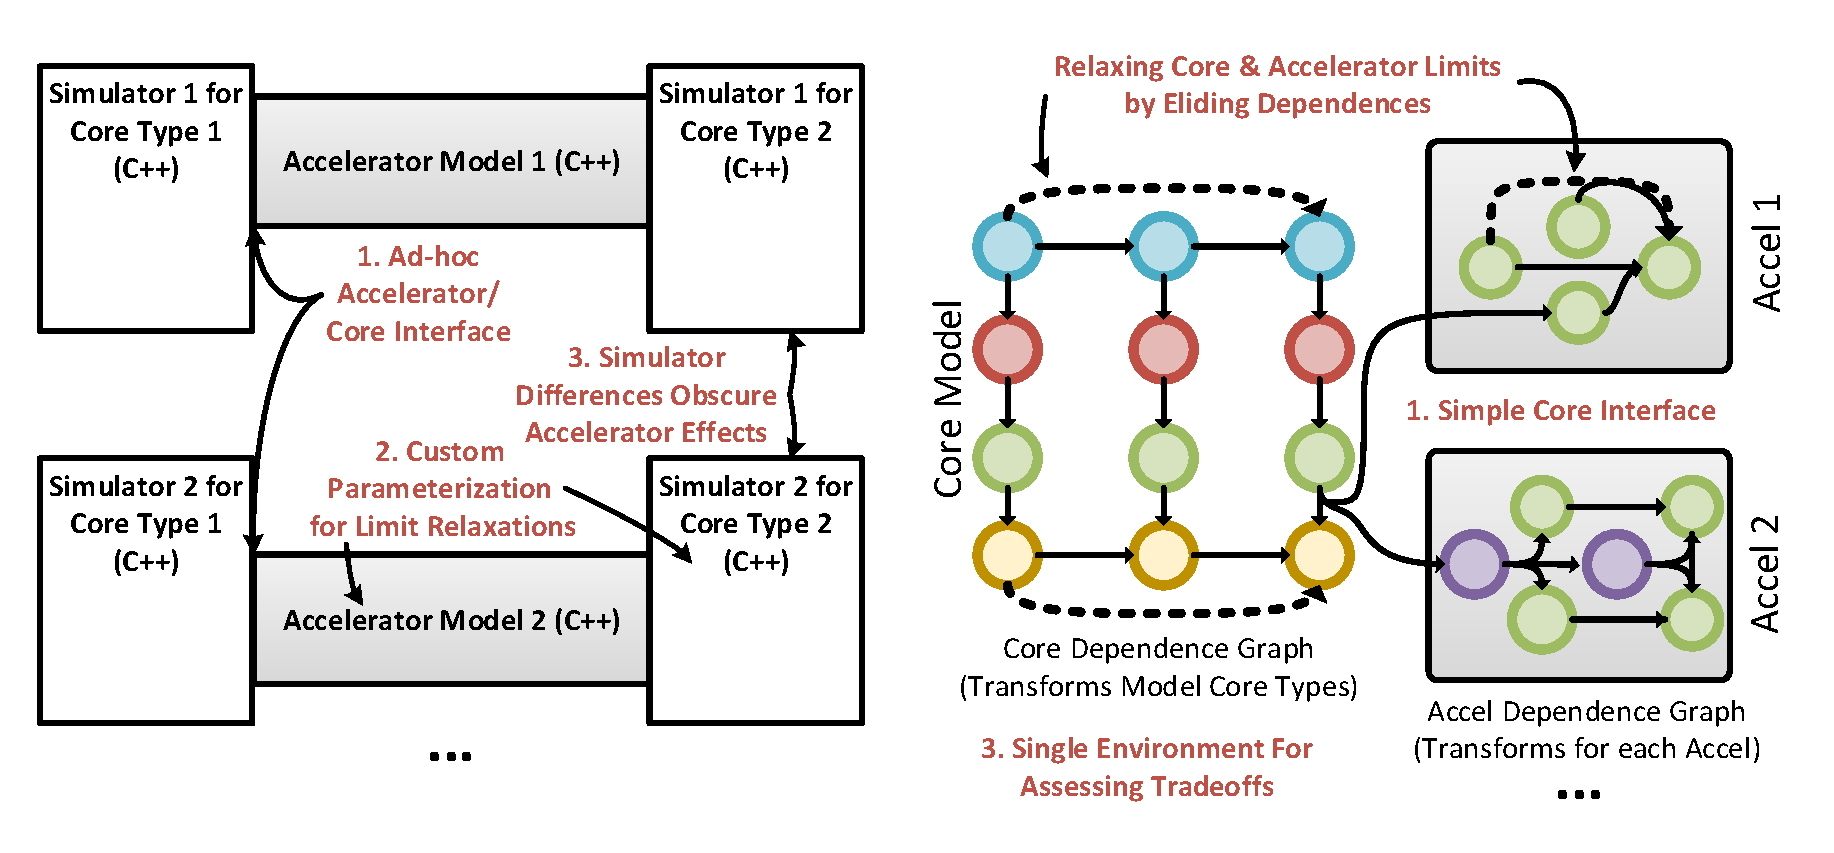
\includegraphics[width=0.85\linewidth]{figs/modeling-overview.pdf}
  \end{center}
\vspace{-0.2in}
  \caption{Current versus proposed approach for finding Limits/Opportunities of Acceleration.}
  \label{fig:modeling-overview}
\vspace{-0.05in}
\end{figure}


\subsection{Motivation}
If the future of performance and energy efficiency entails specialization
through accelerators, then it becomes vital to understand both what
type of accelerators should be developed and what challenges are the most
important to tackle.  Essentially, architects need to know where to look,
and how to spend their time.  As Figure~\ref{fig:modeling-overview} outlines,
this is extremely difficult given the current state of accelerator research,
where different accelerators are implemented in different simulators, requiring
vast effort  in implementation as well as making it difficult to compare results.
The transformable dependence graph (TDG)
is in a unique position to help on this front; it is both abstract and 
can be easily provisioned to model new design choices and forms of acceleration,
and at the same time can accurately capture low level interactions with
the application and with the general purpose processor.  The abstract nature
of the TDG helps in an additional way: we don't need to restrict ourselves to
designs which can be practically built today, we can instead look at the vast array
of architectures which break dependences which we could forseeably invent techniques
for in the future.

What we propose in this direction of research is to describe a set of ``limitations''
which are the primary factors which prevent accelerators from realizing their full
potential performance or energy-efficiency benefits.  These limitations fall under
broad categories like reducing memory serialization or communication with the core,
but will have different hardware implications and expected benefit for different
accelerators.  Implementing TDG models for the different limitations, for the most
part, entails omitting certain nodes and dependence edges.  We are essentially turning
off parts of the models which are already there, where the upper bound model for an
accelerator leaves only the computation nodes, and the data and memory dependences.

We also clarify that the our goal is to explore the limitations and opportunities of
acceleration which can be applied \emph{automatically}, without the aid of a programmer
to revise the application's algorithm. That is, what are the fundamental tradeoffs, 
limitations, and potential benefits of accelerators attainable through automated
processes alone.

\subsection{Research Approach}
After performing detailed analysis across many benchmarks and potential limitations, we
present 9 limitations, both practical and fundamental, explained next, and
outlined in Table~\ref{tab:limitdef}.
The ordering of the transformations will certainly affect the perceived benefit
of each component.  We have attempted to order them in increasing difficulty to
address, which makes sense because it's rational
for designers to address lower hanging fruit first.

%We have performed sensitivity analysis,
%and found that the speedup achieved is potentially more than the sum of the
%components.  For instance, consider accelerating the TPT benchmarks with a
%1-Wide inorder Core + Conservation Cores.  
%The non-unit components of the individual limit relaxations are
%1.4$\times$, 2.2$\times$, 2.8$\times$,1.1$\times$ and 1.3$\times$.  The overall
%speedup is 8.5$\times$, which shows there are more than the sum of accumulative
%effects.

\begin{table}
\footnotesize
\def\arraystretch{1.1}
\setlength{\tabcolsep}{.12em}

\begin{tabular}{>{\RaggedRight}p{0.9in}>{\RaggedRight}p{2.4in}>{\RaggedRight}p{3.2in}}  \toprule
    \textbf{Limit} & \textbf{Description} & \textbf{Parameters} \\ \midrule

    \multicolumn{2}{c}{Practical Limitations}\\ \midrule

    Vector-Fetch Width
    & Amount of data fetched to/from memory with one instruction
    & 4-words, 8-words, 16-words
    \\    

   Accel. Size
   & Area of Accelerator
    (note, these are not normalized to eachother)
   & Beret SEB size: 5,7,9,12;  \ \ 
     SIMD Lanes: 4,8,16 \newline
     C-Cores K-Ops: 0.15,0.5,1,8;
     DySER FUs: 16,25,32,64
   \\

   Mem. \newline Serialization
   & Maximum parallel memory ops.
   & Beret/CCores: 1,2,4,8 Mem Ops per memory region.
   \\

   Core Comm.
   & Overhead of data-transfer.
   & DySER: 3, 1 cycle instructions \& Free \newline
     BERET/C-Cores: 1,2,4 Ops/Cycle
   \\
 
   Accel configuration.
   & Overhead of accelerator configuration time
   & DySER: 64 cycles \& Free \newline
     BERET: 1 cycle per SEB \& free
   \\ \midrule


   \multicolumn{2}{c}{Fundamental Limitations}\\ \midrule
   
   Block Dataflow
   & Acceleration unit blocks are de-serialized.
   & On/Off
   \\

   Full Dataflow
   & Full dataflow for entire acceleratable region.
   & On/Off
   \\

   Execute \newline Specialization
   & Reduces long latency FU access, approximating special function unit integration.
   & 4,1 cycle max latency
   \\   

   Memory \newline Specialization
   & Allows the working set to fit into a particular level of cache.
   & Maximum latency mem access: L2, L1 cache latency
   \\
    
\bottomrule
  \end{tabular}
  \caption{Summary of Limits Considered}
  \label{tab:limitdef}
\vspace{-0.1in}
\end{table}


\paragraph{Practical Limitations}
\begin{itemize}
  \item \textbf{Vector-Fetch Width}
  Vector fetch width is the amount of data which is fetched to or from memory with 
a single instruction. 
%We use 4-word, 8-word, and 16-word length vectors for both the DySER and SIMD models.

\item \textbf{Accelerator Size} In this limitation we vary the most fundamental
aspect of the architecture which affects it's total area.  Note that these are
not normalized to eachother as they are
meant to be a sensitivity parameter. For Conservation Cores we
the number of static operations mapped to hardware.  For DySER, it's size is proportional to the size of the functional unit (FU) grid.  For BERET, the SEB sizes, in terms
of FU count, are considered.  For SIMD the number of compute lanes is the biggest
factor.

\item \textbf{Memory Serialization}
In this limit, we consider the number of allowed parallel memory operations.  
This only pertains to accelerators which do not borrow the main processor
for memory, namely C-Cores and Beret.

\item \textbf{Core Communication}
Here we consider the overhead in communicating values between the 
core and the processor.  For BERET and C-Cores the data transfer model
is calculated in the number of words/cycle.  For DySER, this is the execution
latency of the send/recv instruction.

\item \textbf{Configuration Overhead}
This limit relaxation reduces the overhead time of setting up the accelerator
upon transferring control to the main core.

\end{itemize}


\paragraph{Fundamental Limitations}
\begin{itemize}

\item \textbf{Block Dataflow} Each accelerator executes in ``blocks'' of
computation.  For Conservation Cores this is the basic block, for BERET the
SEB, and for DySER this is the computation subregion.  This relaxation allows
multiple blocks to be executed in parallel, if it isn't already allowed for the
architecture.  Specifically, any ready blocks may fire once the current basic
block has completed.  In practice, while this requires potentially more complex
parallel hardware, it does not impose additional control speculation on the program. 

\item \textbf{Full Dataflow} Full dataflow means that all operations which are
designated to be run on the accelerator are have no other resource or
scheduling restrictions on them.  Note that this assumes enough hardware for
all simultaneous basic blocks to be executing in parallel, as well as facilities
to predict branches.  For BERET this means speculating 
whether loop iterations will be taken, for C-Cores this implies branch prediction.
We assume the C-Cores model has the same type of branch predictor as the
main core, and serialize on a misprediction.

\item \textbf{Execute Specialization}
This relaxation enables long latency functional unit access to be reduced, 
which approximates the benefit of integrating special function unit access 
for relevant computation. We use values of 4 and 1 cycles max FU latency.
 
\item \textbf{Memory Specialization}
This allows the working set of the program to ``fit'' into either L2 or L1 caches.
We implement this by clamping latencies to some max value.
\end{itemize}

\subsection{Preliminary Results}

We first briefly describe some of the basic methodology and setup, 
then discuss preliminary results.

\paragraph{Machine Parameters}
We list here some common machine parameters. We use a 2way set-associative 32KiB I\$ and 
64KiB L1D\$, with a 4 cycle latency, and a 2MB 8-way assoc, L2\$, with a 22 cycle hit latency.  
The core has a 192 entry ROB, 64 entry IW, 32 entry LSQ, and 2 load/store ports.
The four-issue OOO core has 3 ALUs, 2FPs, and 1 Mul/Div unit, 
which are scaled to various issue widths.
For power and energy, we use the $22nm$ setting in McPAT.  
%Validation
%for BERET and Conservation Cores is performed at $65nm$ and $45nm$ respectively.

\paragraph{Benchmarks}
We selected benchmarks from several suites, including throughput
kernels from~\cite{ieeemicro12:dyser}.
MediaBench~\cite{645830}, Parboil~\cite{parboil}, and SPEC INT,
which are listed in Table~\ref{tab:benchmarks}.  
This set of benchmarks covers applications from many domains, and
their diversity serves to demonstrate application-accelerator interaction.

\begin{table}
\footnotesize
\begin{center}
\def\arraystretch{0.95}
\setlength{\tabcolsep}{.19em}

    \begin{tabular}{l>{\RaggedRight}p{4.0in}}  \toprule
    \textbf{Suite} & \textbf{Benchmarks} \\ \midrule
    TPT & 
      conv,  merge,  nbody,  radar,  treesearch,  vr \\ 
    Parboil & 
      cutcp,  fft,  kmeans,  lbm,  mm,  needle,  nnw,  spmv,  stencil,  tpacf\\ 
    Mediabench & 
      cjpeg,  djpeg,  gsmdecode,  gsmencode   cjpeg2,  djpeg2,  h263enc,  h264dec,  jpg2000dec,  jpg2000enc,  mpeg2dec,  mpeg2enc  \\ 
    SPEC INT & 
      164.gzip,  181.mcf,  175.vpr,  197.parser,  256.bzip2   429.mcf,  403.gcc,  458.sjeng,  473.astar,  456.hmmer \\ 
    NPU Suite & 
      fft, inversek2j, jmeint, jpeg, kmeans, sobel\\ 

\bottomrule
  \end{tabular}
\end{center}
\vspace{-0.2in}

  \caption{Benchmarks}
  \label{tab:benchmarks}
\end{table}




\begin{figure*}
\begin{adjustwidth}{-1.1in}{-1.1in}
\begin{center}

\begin{tabular}{m{0.01\linewidth}m{0.98\linewidth}}
%\parbox[t]{-1mm}{\rotatebox[origin=c]{90}{\textbf{Performance}}} & 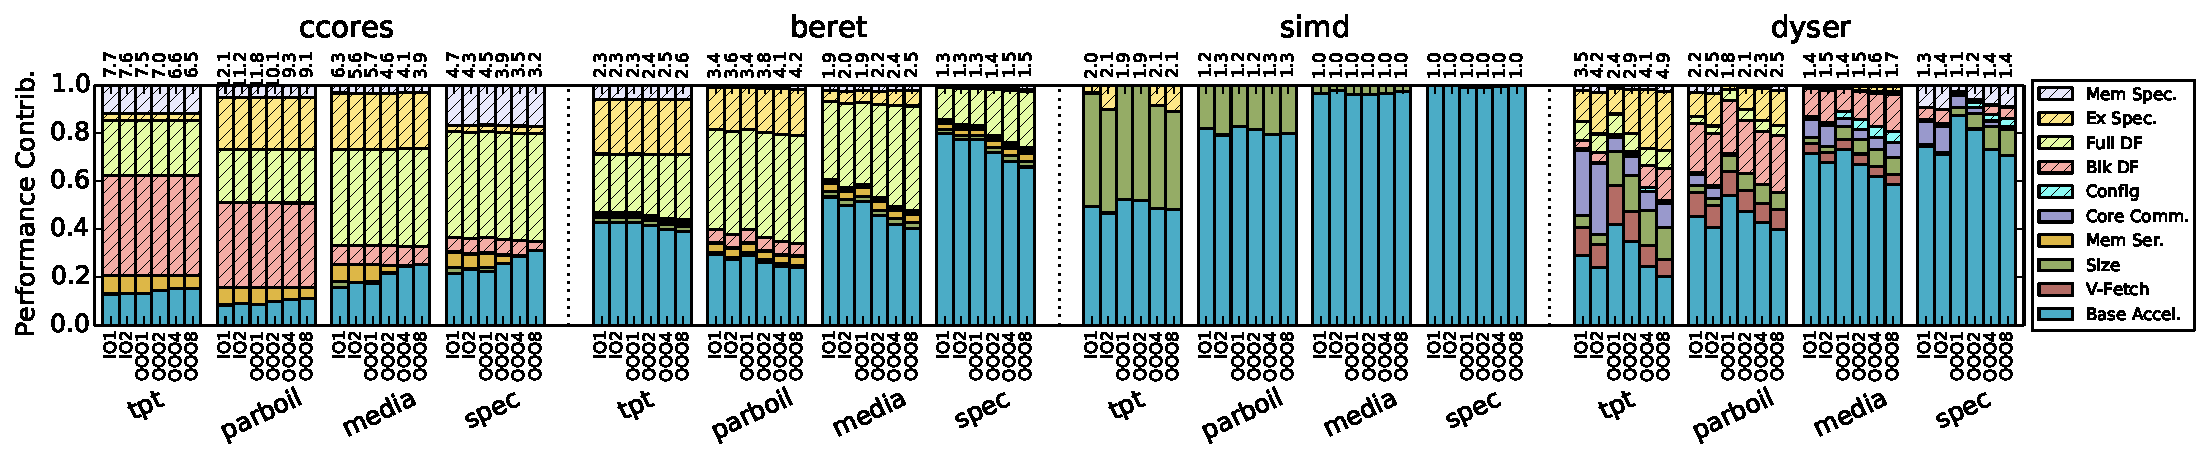
\includegraphics[width=0.95\linewidth]{figs/full-limits-Performance.pdf}  \\
 
%\parbox[t]{-1mm}{\rotatebox[origin=c]{90}{\textbf{Energy}}} & 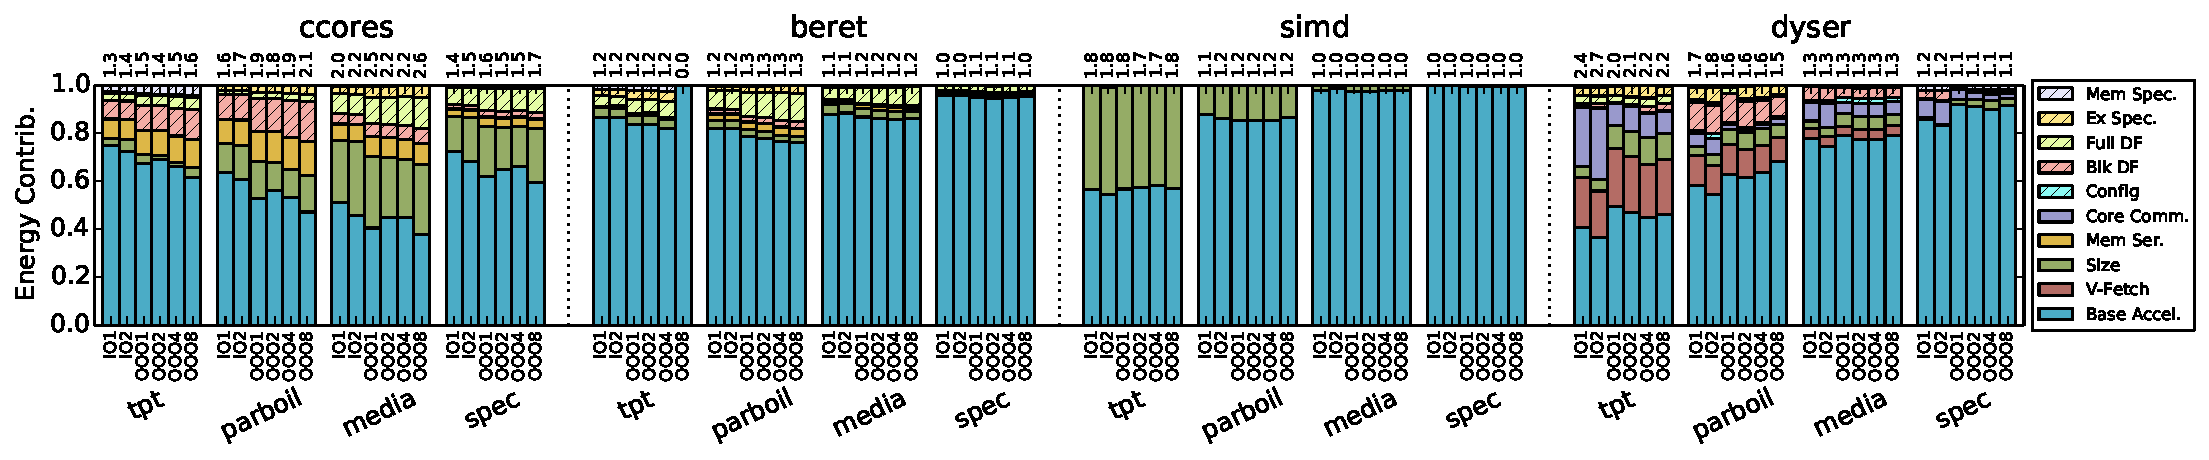
\includegraphics[width=0.95\linewidth]{figs/full-limits-Energy.pdf}  \\

\parbox[t]{-1mm}{\rotatebox[origin=c]{90}{\textbf{}}} & 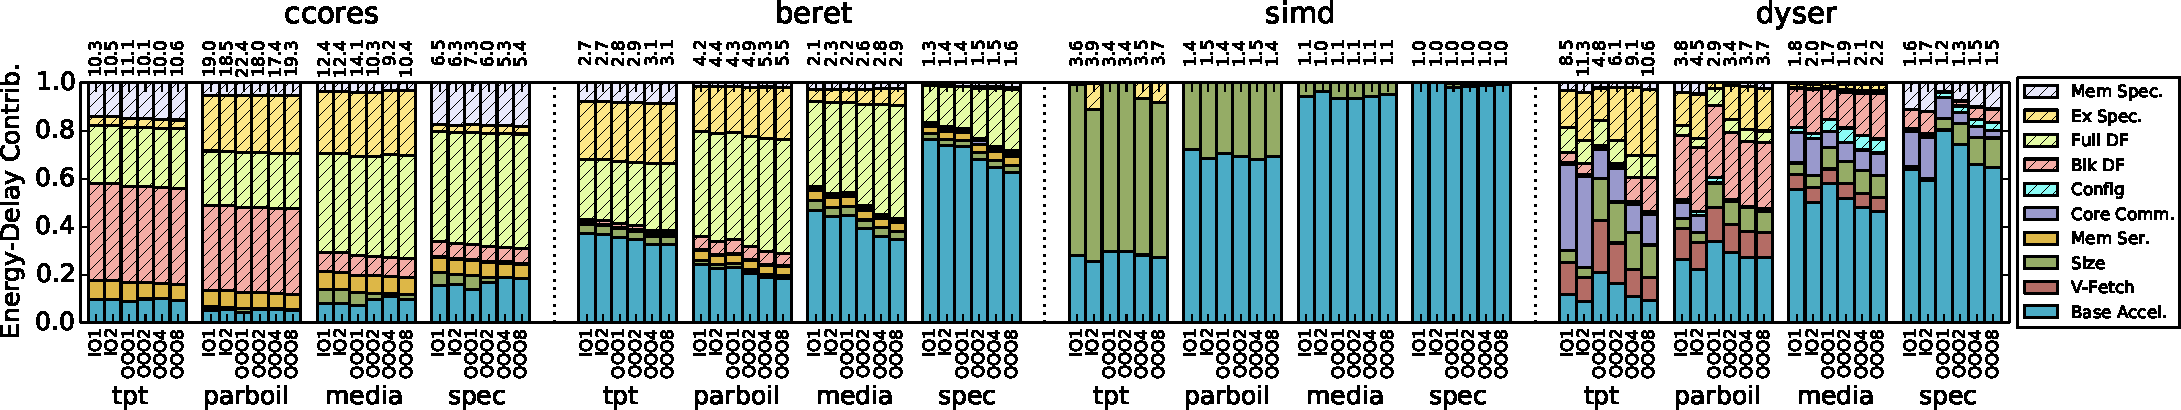
\includegraphics[width=0.95\linewidth]{figs/full-limits-Energy-Delay.pdf}  \\
\end{tabular}
\vspace{-0.18in}
\end{center}
\end{adjustwidth}
\caption{Impact of Limit-Relaxations for all Cores/Accelerators/Benchmark suites, in terms of normalized energy delay.  Numbers above bars indicate maximum energy-delay achievable.}
\vspace{-0.1in}
\label{fig:enDelay}
\end{figure*}




\begin{figure}
\begin{center}
\footnotesize
\def\arraystretch{0.02}
\setlength{\tabcolsep}{0.1em}

\begin{tabular}{m{0.26\linewidth}m{0.34\linewidth}}
\multicolumn{2}{c}{(a) Opportunities over all workloads}\\
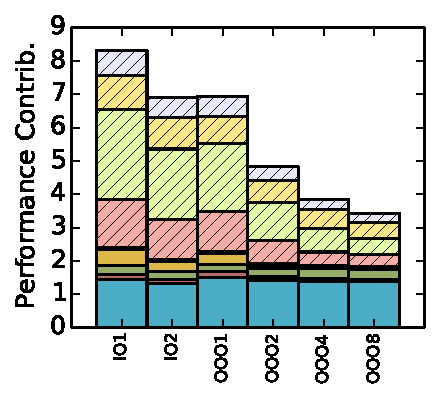
\includegraphics[width=0.99\linewidth]{figs/opportunities-Performance-normal.pdf} &
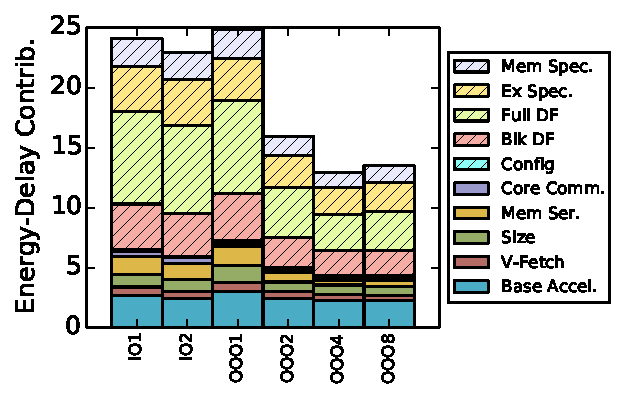
\includegraphics[width=0.99\linewidth]{figs/opportunities-Energy-Delay-normal.pdf} \\

\multicolumn{2}{c}{(b) Per-Benchmark Potential Acceleration Speedup}\\
\multicolumn{2}{c}{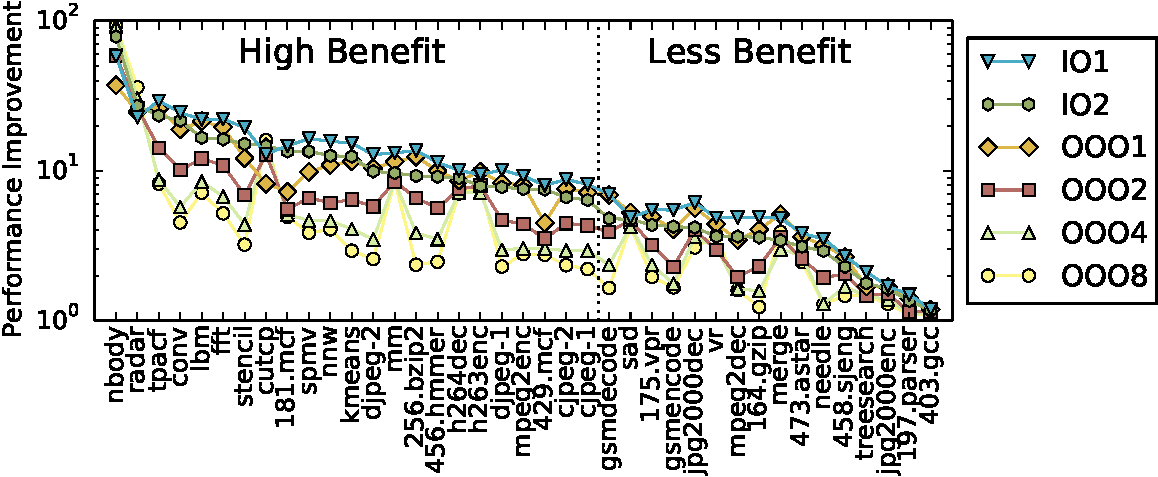
\includegraphics[width=0.6\linewidth]{figs/bench_opportunity9.pdf}} \\

\multicolumn{2}{c}{(c) Opportunities over high-benefit workloads}\\
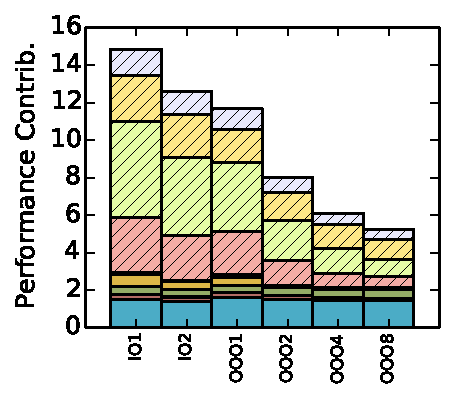
\includegraphics[width=0.99\linewidth]{figs/opportunities-Performance-super.pdf} &
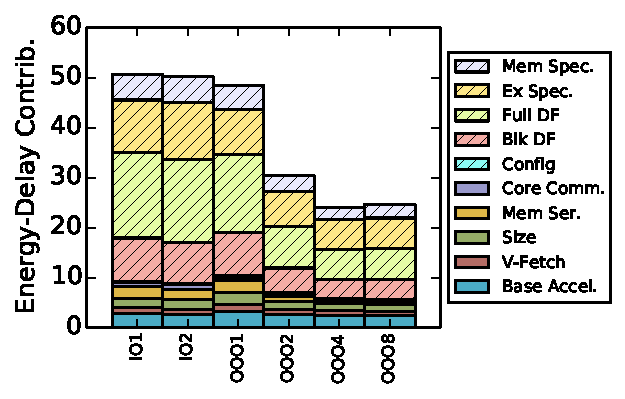
\includegraphics[width=0.99\linewidth]{figs/opportunities-Energy-Delay-super.pdf}
\end{tabular}
\vspace{-0.1in}
\caption{Opportunities across all Benchmarks}
\label{fig:oppo}  
\end{center}
\vspace{-0.2in}
\end{figure}





\paragraph{Cross Product Results}
Figure~\ref{fig:enDelay} shows summary of the limit study between the cross
product of benchmark, general purpose core and accelerator, using the metric
of energy-delay.  On the y-axis is the percentage of total improvement which 
each limit relaxation provides, and the number above each bar is the total 
improvement.  

The first observation is that
relaxations have different effects on different benchmark suites.  For conservation
cores on data-parallel benchmarks like TPT and PARBOIL, enabling block dataflow
is enough to see 3$\times$ improvements in energy-delay.  The same architecture
with SPEC INT, which has much more frequent control flow, needs full-dataflow to be
effective.  Also, while one would expect the benefit of relaxations to be independent
of the GPP core type, this is clearly not always the case.  Considering the DySER
accelerator, we can see that the core communication bottleneck can provide huge
improvements on certain benchmarks, especially on the inorder-core types.

\paragraph{Benefits of Multi-acceleration}
By combining multiple accelerators together, it's possible to see significantly
more benefit than from just a single design alone.  The true potential
for acceleration lies in the ability to combine techniques, achieving the benefits of 
heterogeneity on a much more fundamental basis than just microarchtiectural changes.
To see the potential benefits of such an approach, Figure~\ref{fig:oppo}(a) 
shows the geometric mean improvement when considering the best possible 
acceleration for each benchmark, relative to its baseline general purpose
core for each relaxation
we consider. Figure~\ref{fig:oppo}(b) shows the potential performance 
improvement for each core type on each benchmark, considering the best accelerator for each.  If we consider benchmarks with over 5$\times$ speedup on inorder cores as 
``high-benefit'' benchmarks, then Figure~\ref{fig:oppo}(c) shows the improvement
of acceleration on these.  

Here we can see that reducing serialization, both inside and across accelerator
unit blocks, is hugely important and can lead to significant improvements in
both energy and energy delay.  To summarize the results, across all benchmarks,
the multi-accelerator potential is up to 3.5$\times$ and 8$\times$ performance
for OOO and inorder cores, and up to 13$\times$ and 25$\times$ respectively for
Energy-Delay.  For high benefit workloads, the potential is 5$\times$ and
14$\times$ performance on OOO and inorder cores, and up to 30$\times$ and
50$\times$ for Energy-Delay.

\subsection{Proposed Work} 

\paragraph{Additional Experiments \& Analysis}
While we have merely scratched the surface in this proposal, our ultimate aim is
to comprehensively address the following five questions about the nature of acceleration.
\begin{inparaenum}
\item What are accelerator's fundamental limitations?
\item What are the potential benefits of multi-accelerator systems?
\item By how much does the baseline general purpose core matter?
\item Is the metric important in choosing an accelerator? 
\item What accelerators are effective in which domains?
\end{inparaenum}
Using the transformable dependence graph is an appropriate approach, because
it does direct modeling of the execution of an accelerator on a benchmark
as well as modeling the GPP, so in can capture application and core interactions,
and also is abstract enough to be flexible in modeling.  The experiments for
questions 4 \& 5 are mostly explained.  For questions 1-3, we will pick a specific
design point for each accelerator, and then vary the applications and baseline cores,
and analyze the behavior of the models to find patterns.

\paragraph{Formalizing Transformations}
We also propose to more 
formally define the semantics of the graph transformations for modeling 
accelerators and performing limit studies. This work so far essentially 
describes how the graph is changed by a transformation,
and would be significantly improved by a more formal algorithmic description of 
the transformation procedure.  Even better would be to describe the transformations
in such a way that they can be guaranteed to be correct, even when composed in
some ordering.  While it's not certain whether a framework such as this exists,
its possibility merits exploration.


\subsection{Related Work} \label{sec:related}

\paragraph{Modeling}
Many recent papers have presented a case for specialization and
heterogeneity using analytical
models~\cite{Chung:2010,6336691,Navigo}, high-level technology trend
projections~\cite{DBLP:journals/cacm/BorkarC11,6164927}, or by
modeling general purpose processors~\cite{isca11:dark-silicon}.
Models for heterogeneous execution
include~\cite{boat-hull1,boat-hull0,Williams:2009:RIV:1498765.1498785,
  Hong:2010:IGP:1815961.1815998,hongkimperf2,meng2011grophecy,Wang:2009:PMR:1616625.1616631,6114198},
which are related to analytical models for general purpose
processors~\cite{Eyerman:2009:MPM:1534909.1534910,doi:10.2200/S00273ED1V01Y201006CAC010}.
These are specific to one accelerator or general-purpose core
performance and do not allow projection of other metrics like power
and energy or limit studies. Cascaval et al. introduce a taxonomy and
outline some opportunities of acceleration~\cite{Cascaval:2010:TAA:1940702.1940705}.


\paragraph{Quantitative/Limit studies}
% Hameed~\cite{1815968} et al. present a detailed analysis of
% general-purpose processing to motivate specialization by considering
% one example application - media processing.  They conclude that
% detailed algorithmic understanding is required to get 100X and higher
% improvements.
 Azizi et al. present a cost analysis framework of
optimal general purpose processors from an energy and performance
perspective~\cite{Azizi:2010:ETP:1815961.1815967}.  In the previous
decade, Agarwal et al. presented a study on fundamental limits of OOO
microprocessors~\cite{Agarwal01:ISCA}, and preceding that, the limits
of ILP~\cite{Wall:1991:LIP:106972.106991}. Our work, is a
reincarnation of  Wall's ILP study for today's accelerators/heterogeneity driven design paradigm.
